\begin{figure}[t]
% \def\bb{\rule{2in}{0pt}\rule{0pt}{1in}}
\def\topbtm{5cm}
\centering
% \resizebox{.95\linewidth}{!}{
    \center{
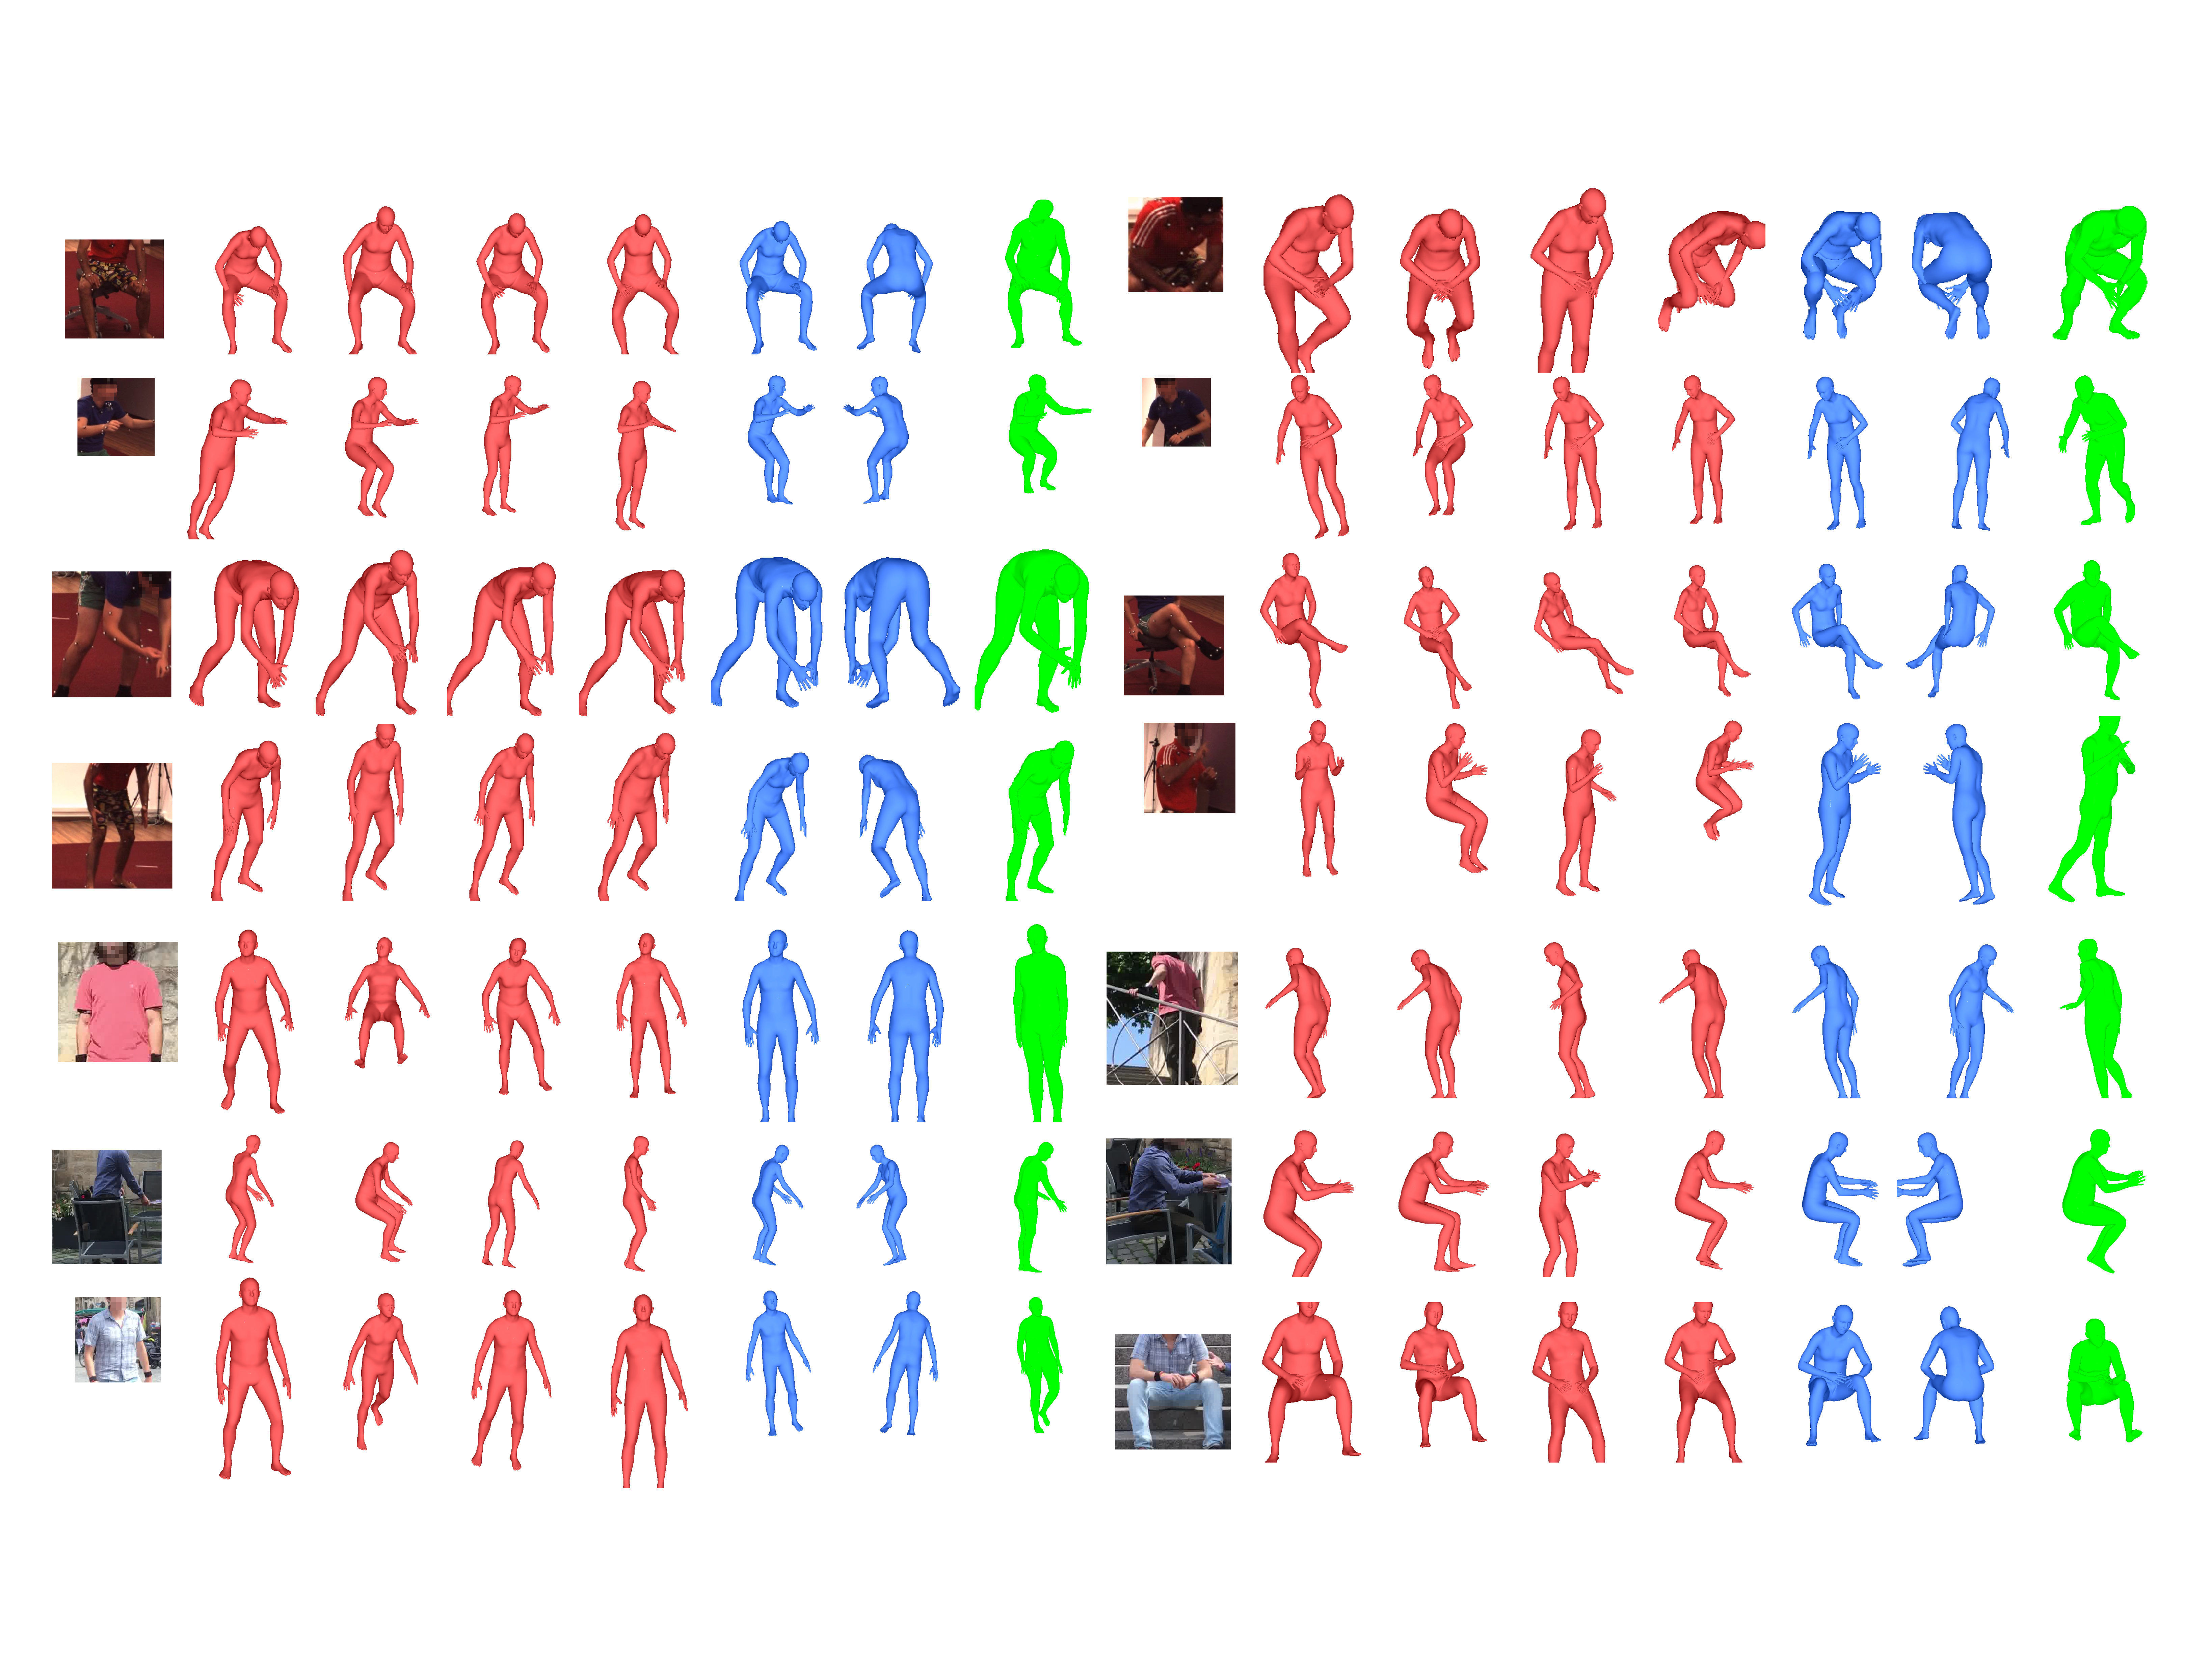
\includegraphics[trim=0.4cm 1cm 8.15cm 1cm,clip,width=0.95\linewidth]{exps/qual_results_all/qualfigs_3.png}
    }

% }
% \vspace{-1.15cm}
\caption{%
    \textbf{Qualitative results from $n=5$ quantization on monocular mesh recovery on AH36m and A3DPW.} 
    From left to right, each group of figures depicts the input ambiguous image, five network hypotheses with the closest to the ground truth in blue, and the ground truth pose in green.
    }\label{fig:qual_results_all}
\end{figure}


\begin{figure}[t]
% \def\bb{\rule{2in}{0pt}\rule{0pt}{1in}}
\centering
% \resizebox{.95\linewidth}{!}{
    \center{
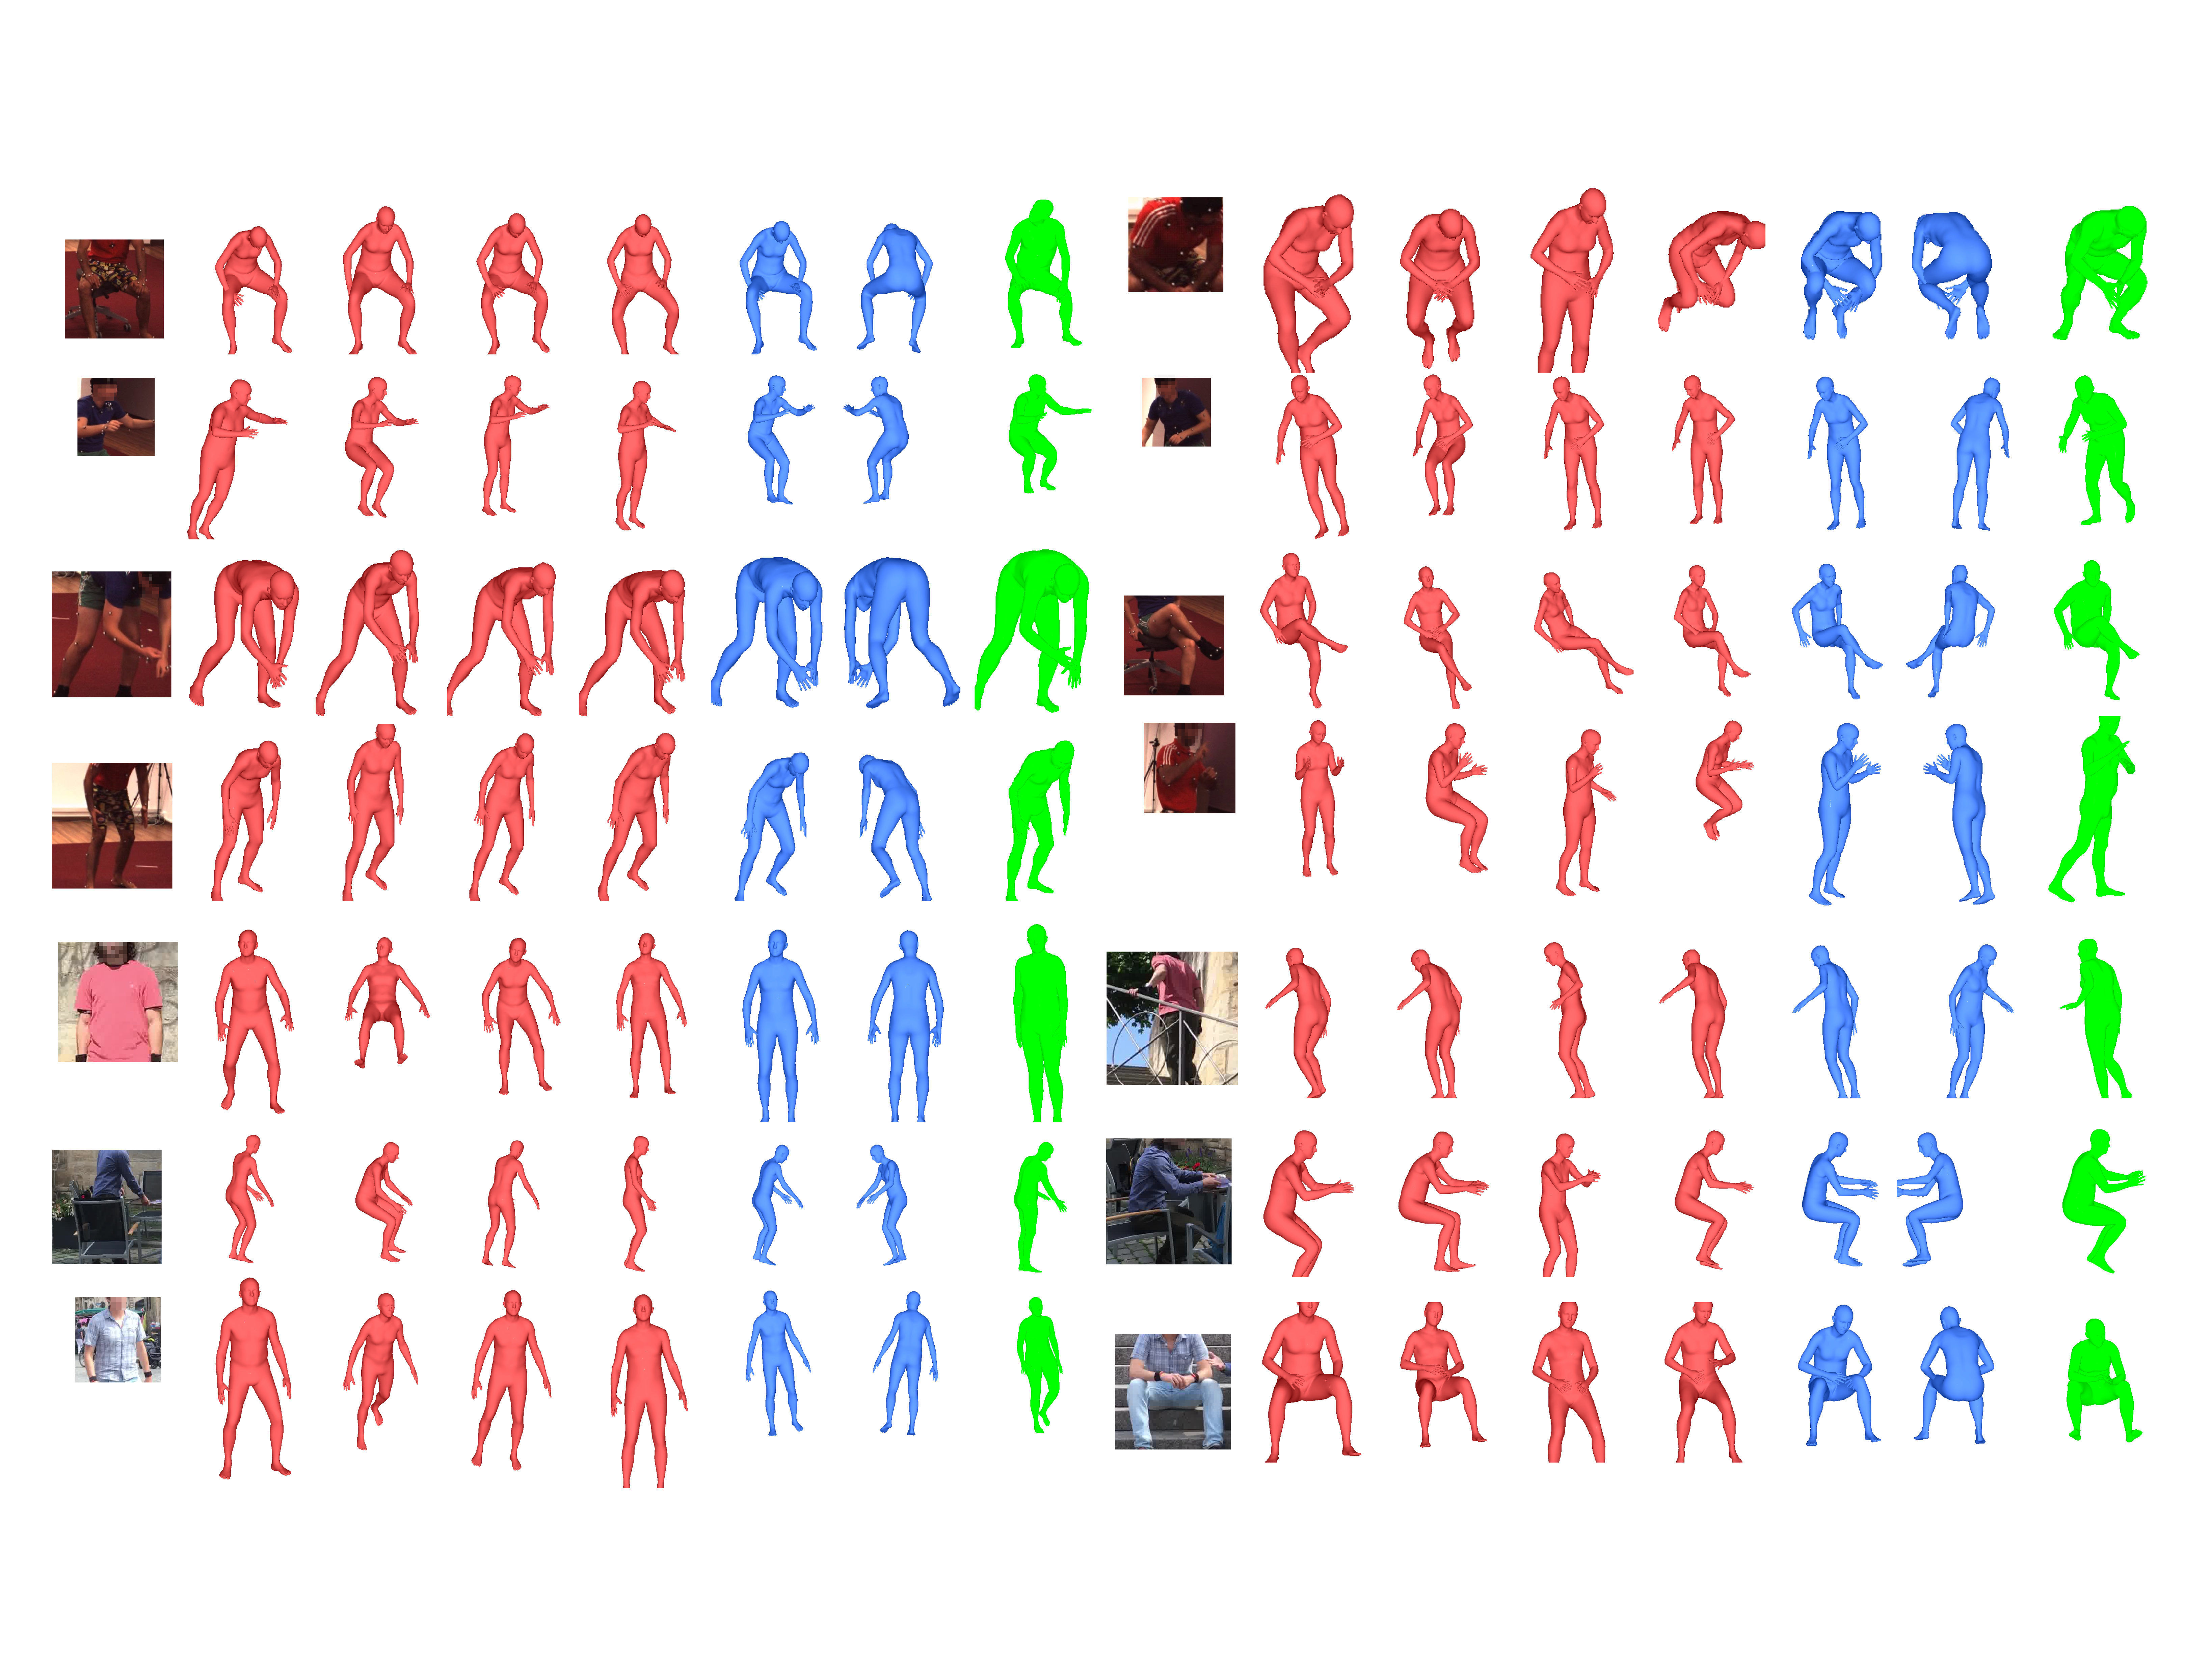
\includegraphics[trim=8.15cm 1cm 0.4cm 1cm,clip,width=0.95\linewidth]{exps/qual_results_all/qualfigs_3.png}
    }
% }
% \vspace{-1.15cm}
\caption{%
    \textbf{Qualitative results from $n=5$ quantization on monocular mesh recovery on AH36m and A3DPW (continued).} 
    From left to right, each group of figures depicts the input ambiguous image, five network hypotheses with the closest to the ground truth in blue, and the ground truth pose in green.
    }\label{fig:qual_results_all2}
\end{figure}